\chapter[Resultados]{Resultados}
Este capítulo apresenta os resultados obtidos. Eles serão apresentados sendo
correlacionando aos objetivos específicos, indicados na Seção \ref{objspec}.
Para cada objetivo foi gerado uma seção neste capítulo.

\section{Identificação de Regras Gramaticais da Linguagem Alvo Inicial}
A linguagem escolhida como alvo inicial do \textit{framework} desenvolvido
neste trabalho foi o \textsf{Grails}. \textsf{Grails}, antigamente conhecido
como \textsf{Groovy on Rails}, é um \textit{web framework} para plataforma Java
\cite{grails2015}. Para melhor entender a sintaxe da linguagem de programação
alvo, partiu-se da documentação oficial do \textsf{Groovy}, com o intuito de
aprofundar-se o conhecimento sobre as regras gramaticais do alvo inicial do
\textit{framework}.

Para a identificação das regras gramaticias foram selecionadas duas ferramentas,
bastante utilizadas em contextos de desenvolvimento de compiladores e
\textit{parsers}: \textsf{Flexc++} e \textsf{Bisonc++}. Ambas as ferramentas, \textsf{Flexc++} e \textsf{Bisonc++} foram desenvolvidas por Frank B. Brokken, gerente de segurança em TI e conferencista na \textit{University of Groningen}, Holanda.

A primeira ferramenta foi utilizada para definir \textit{scanners}, cujo propósito é a identificação de padrões léxicos em um arquivo de texto. Esses padrões foram definidos a partir de \textit{regex}, na primeira seção do arquivo fonte do Flexc++. Na próxima seção definiu-se o que acontece quando um dos padrões é identificado. No Código \ref{fragflexcpp} demonstra-se um fragmento do arquivo produzido para a execução do \textsf{Flexc++}.

\begin{lstlisting}[language=C++, label=fragflexcpp, caption=Fragmento do código fonte para o \flexcpp]
TRUE    true (*@\label{fragflexcpp1}@*)
FALSE   false (*@\label{fragflexcpp2}@*)
BOOLEAN {TRUE}|{FALSE} (*@\label{fragflexcpp3}@*)

%x oneline_string (*@\label{fragflexcpp5}@*)
%x multiline_string (*@\label{fragflexcpp6}@*)
%x multiline_comment (*@\label{fragflexcpp7}@*)


%%

"class" { (*@\label{fragflexcpp12}@*)
  *d_val = matched(); (*@\label{fragflexcpp13}@*)
  return Parser::CLASS; (*@\label{fragflexcpp14}@*)
}
\end{lstlisting}

Observa-se no Código \ref{fragflexcpp}, entre as linhas \ref{fragflexcpp12} e \ref{fragflexcpp14}, um exemplo de como o \textsf{Flexc++} é usado:
define-se um padrão léxico a ser encontrado no texto linha (\ref{fragflexcpp12}) e
a ação a ser executada para aquele padrão. No caso exemplificado, o
padrão a ser encontrado é a palavra \textsf{class}. Assim, quando o Flexc++
identifica essa palavra ele armazena o resutado da comparação entre a palavra em
análise e o padrão definido (linha \ref{fragflexcpp13}). Caso haja correspondência o
Flexc++ retorna um \textit{token} definido no arquivo gerado pelo
\textsf{Bisonc++} (linha \ref{fragflexcpp14}).

Um outro recurso do \textsf{Flexc++} utilizado para a identificação das regras
gramaticais do \textsf{Grails} foi a definição de \textit{mini scanners}. É um
recurso fornecido pelo \textsf{Flexc++} que permite a definição de \textit{scanners}
com regras mais específicas dentro do \textit{scanner} maior. Isso foi útil para
definir os padrões de identificação de \textit{strings} e comentários do alvo inicial deste trabalho.

O Código \ref{miniscanner} apresenta o \textit{mini scanner} definido para
identificação de \textit{strings}.

\begin{lstlisting}[language=C++, label=miniscanner, caption=Implementação do Mini scanner de Strings]
// Condição inicial para o mini scanner
"\'\'\'" |
"\"\"\"" {
  more();
  begin( StartCondition__::multiline_string );
}


// Mini scanner e suas regras
<multiline_string> {
  "\'\'\'"  |
  "\"\"\"" {
    begin( StartCondition__::INITIAL );
    *d_val = matched();
    return Parser::STRING;
  }

  .|\n {
    more();
  }
}
\end{lstlisting}

O uso de \textit{mini scanners} é semelhante ao \textit{scanner} comum. É
importante ressaltar que há dois tipos de \textit{mini scanners}: os exclusivos
e o inclusivos. Um \textit{mini scanner} inclusivo permite a inclusão de novos
padrões ao identificador a partir do momento em que este é chamado. Já o
\textit{exclusivo} cessa as atividades das regras definidas pelo \textit{scanner}
e faz valer apenas as definidas por ele. Para este trabalho foram definidos apenas
\textit{mini scanners} exclusivos. Além disso, \textit{mini scanners} possuem
duas funções a mais: a \textit{StartCondition\_\_::[nome do mini scanner]}, que
inicia o \textit{mini scanner}, e a \textit{StartCondition\_\_::INITIAL} que
finaliza seu uso. Quando o \textit{scanner} encontra no texto em análise o
padrão que dá início a um \textit{mini scanner}, ele para o seu processo e
inicia o do \textit{mini scanner}. Assim, apenas as regras do \miniscanner passam a ser
válidas. No momento que o \textit{miniscanner} encontra o padrão de finalização
ele retoma o processo do \textit{scanner}.

Em conjunto com o \textsf{Flexc++} foi utilizado o \textsf{Bisonc++}. Como já
apresentada, a primeira ferramenta identifica padrões léxicos, enquanto que a
segunda ferramenta é responsável pela definição das regras sintáticas da
gramática.

Da mesma forma que o \textsf{Flexc++}, o arquivo a ser compilado pelo \bisoncpp é divido
em duas seções. A primeira traz algumas diretivas que fornecem infomações ao
\bisoncpp sobre configurações e opções que serão adicionadas ao código fonte
gerado pela ferramenta. A segunda parte desse mesmo arquivo traz as regras
que definem a gramática. O Código \ref{fragbisoncpp} descreve um fragmento
do arquivo com a implementação das regras gramaticais do \textsf{Grails}.

\begin{lstlisting}[language=C++, label=fragbisoncpp, caption=Fragmento do código fonte para o \bisoncpp]
// Seção de diretivas
%scanner                  ../scanner/Scanner.h (*@\label{fragbisoncpp1}@*)
%scanner-token-function   d_scanner.lex() (*@\label{fragbisoncpp2}@*)
%baseclass-preinclude     ParserPreinclude.h (*@\label{fragbisoncpp3}@*)

%stype std::string (*@\label{fragbisoncpp5}@*)
%start startrule (*@\label{fragbisoncpp6}@*)

%include spec/tokens.y (*@\label{fragbisoncpp8}@*)

%%


// Definição de uma das regras gramaticais do Grails
class_definition: (*@\label{fragbisoncpp14}@*)
  CLASS IDENTIFIER { (*@\label{fragbisoncpp15}@*)
    std::string identifier_token( (*@\textdollar@*)2 ); (*@\label{fragbisoncpp16}@*)
    collector->collect_data( "c", identifier_token.c_str() ); (*@\label{fragbisoncpp17}@*)
  }
| ABSTRACT class_definition (*@\label{fragbisoncpp18}@*)
| class_definition class_complements (*@\label{fragbisoncpp19}@*)
;
\end{lstlisting}

Como dito anteriormente, na primeira parte do arquivo foram utilizadas algumas
diretivas do \bisoncpp que forneceram opções úteis para o desenvolvimento do
\parser e, consequentemente, da identificação das regras gramaticais. Das
diretivas apresentas entre as linhas \ref{fragbisoncpp1} e
\ref{fragbisoncpp8}, as que merecem menção são a da linha
\ref{fragbisoncpp1}, que indica o \scanner que foi utilizado,
a \ref{fragbisoncpp2}, que indica de onde serão lidas as palavras identificadas
pelo \textit{scanner}, e a linha \ref{fragbisoncpp8}, que inclui um outro
arquivo contendo os \tokens utilizados na construção da gramática.

Entre as linhas \ref{fragbisoncpp14} e \ref{fragbisoncpp19} do Código
\ref{fragbisoncpp}, pode-se observar uma das regras construídas neste trabalho.
A linha \ref{fragbisoncpp14} indica o nome da regra a ser construída, o que
gera a adição de um novo símbolo não terminal, chamado
\lstinline|class_definition|. Essa nova regra possui três definições possíveis,
listadas nas linhas \ref{fragbisoncpp15}, \ref{fragbisoncpp18} e
\ref{fragbisoncpp19}. É importante observar que as definições de regras no
\bisoncpp são recursivas. Dessa forma, definiu-se uma definição base para a
\lstinline|class_definition| que foi reutilizada nas outras duas possibilidades.
As linhas \ref{fragbisoncpp16} e \ref{fragbisoncpp17} são as ações que foram
implementandas para serem executadas quando essa regra for identificada.
No caso, a linha \ref{fragbisoncpp16} captura o token e o atribui a uma \str,
enquanto que a linha \ref{fragbisoncpp17} faz a coleta da
palavra encontrada na segunda posição da regra. A coleta de dados foi explicada na
seção anterior, sobre o \Scarefault.

\flexcpp e \textsf{Bisonc++}, quando executados, geram duas classes escritas
em C++.
É necessário fazer a comunicação entre o analisador léxico, produzido pelo
\textsf{Flexc++}, com o analisador sintático gerado pelo \textsf{Bisonc++}.
Para isso, foi necessário a criação de um ponteiro dentro do analisador
léxico que apontasse para um atributo especial no analisador sintático.
Assim, a comunicação entre ambos os módulos foi possível.

No Código \ref{talk-FB-scannerh} apresentam-se as alterações feitas no
arquivo \lstinline|Scanner.h|. Na linha \ref{scannerh11} foi adicionado um atributo,
do tipo ponteiro, com a finalidade de receber a localização de um atributo especial
do \textit{parser}. Para atribuir valores a esse atributo foi definida uma
função membro, linha \ref{scannerh7}, e sua implementação, linha \ref{scannerh14}.
\begin{lstlisting}[language=C++, label=talk-FB-scannerh, caption=Alterações no Scanner.h para comunicação entre Analisador Léxico e Sintático]
#include "../parser/Parserbase.h"

class Scanner: public ScannerBase
{
  public:
  [...]
  void setSval(Parser::STYPE__* d_val__); (*@\label{scannerh7}@*)

  private:
  [...]
  Parser::STYPE__* d_val; (*@\label{scannerh11}@*)
};

inline void Scanner::setSval(Parser::STYPE__* d_val__) (*@\label{scannerh14}@*)
{
  d_val = d_val__;
}
\end{lstlisting}

No Código \ref{talk-FB-parserh} obseva-se as alterações feitas no arquivo
\lstinline|Parser.h| para que houvesse a comunicação com o \lstinline|Scanner.h|.
Na linha \ref{parserh6} declarou-se um objeto do tipo
\lstinline|Collector::CollectorBase *|, cuja função é explicada mais adiante.
Na linha \ref{parserh7} é declarado o objeto responsável pelas mensagens de
\textit{log}, enquanto que na linha \ref{parserh10} declarou-se um novo
construtor para o Parser.
\begin{lstlisting}[language=C++, label=talk-FB-parserh, caption=Alterações no Parser.h para comunicação entre Analisador Léxico e Sintático]
#include "../scanner/Scanner.h"

class Parser: public ParserBase
{
  Scanner d_scanner;
  Collector::CollectorFactory * factory; (*@\label{line:decl-factory}@*)
  Collector::CollectorBase * collector; (*@\label{parserh6}@*)
  LogSystem::Log log; (*@\label{parserh7}@*)

  public:
    explicit Parser(Collector::Language, (*@\label{parserh10}@*)
    					std::istream &in = std::cin,
    					std::ostream &out = std::cout);
  [...]
};
\end{lstlisting}

No Código \ref{talk-FB-parserih} mostra-se a implementação do construtor.
Permite-se, assim, ao objeto \lstinline|d_scanner| conhecer o endereço
de \lstinline|d_val__|, garantindo a comunicação entre o analisador léxico e
sintático. Além disso, é nesse construtor que se instanciou o coletor de
dados.
\begin{lstlisting}[language=C++, label=talk-FB-parserih, caption=Alterações no Parser.ih para comunicação entre Analisador Léxico e Sintático]
#include "Parser.h"

Parser::Parser(Collector::Language language,
			   std::istream &in, std::ostream &out)
{
   d_scanner.switchStreams( in );
	 d_scanner.setSval(&d_val__);
	 factory = new Collector::CollectorFactory();
   collector = factory->get_collector(language);
}

[...]
\end{lstlisting}

Tendo as regras gramaticais sido analisadas e construídas fazendo-se uso
do \flexcpp e do \textsf{Bisonc++}, foram feitos diversos testes manuais
de identificação da linguagem \grails como uso do \parser e do \scanner
gerados. Esses testes deram-se por meio da execução do \parser sobre um
arquivo fonte escrito em \textsf{Grails}. Quando a execução finalizava
observava-se se algum erro de sintaxe era encontrado. Para tornar esse
tipo de teste de identificação das regras gramaticais melhores, foi
implementado um \textit{script} que faz a comparação entre o arquivo de
\textit{log} gerado e um arquivo contendo as mensagens esperadas após
a execução do \parser utilizando três código fonte.

Mesmo sendo capaz de identificar grande porção das regras gramaticais da
linguagem \textsf{Grails}, o \parser ainda não é capaz de identificar todas
as regras definidas para essa linguagem. Algumas especificidades, como alguns
operadores, exemplo o \textsf{elvis}, e cadeias de expressões contidas
em parênteses. Ao adicionar essas regras alguns conflitos do tipo
\lstinline|reduce/reduce| eram reportados, o que inviabilizava o
prosseguimento da implementação. Foram efetuadas diversas pesquisas
sobre como resolver esse tipo de conflito numa gramática, mas não foi
obtido sucesso. Optou-se por dar continuidade nos trabalhos, mesmo sem
cobrir por completo a gramática.

A Figura \ref{identification-test} apresenta o resultado da execução do
\textit{script} de teste de identificação das regras gramaticais definidas
para o \textsf{Grails}.
\begin{figure}[h]
  \centering
    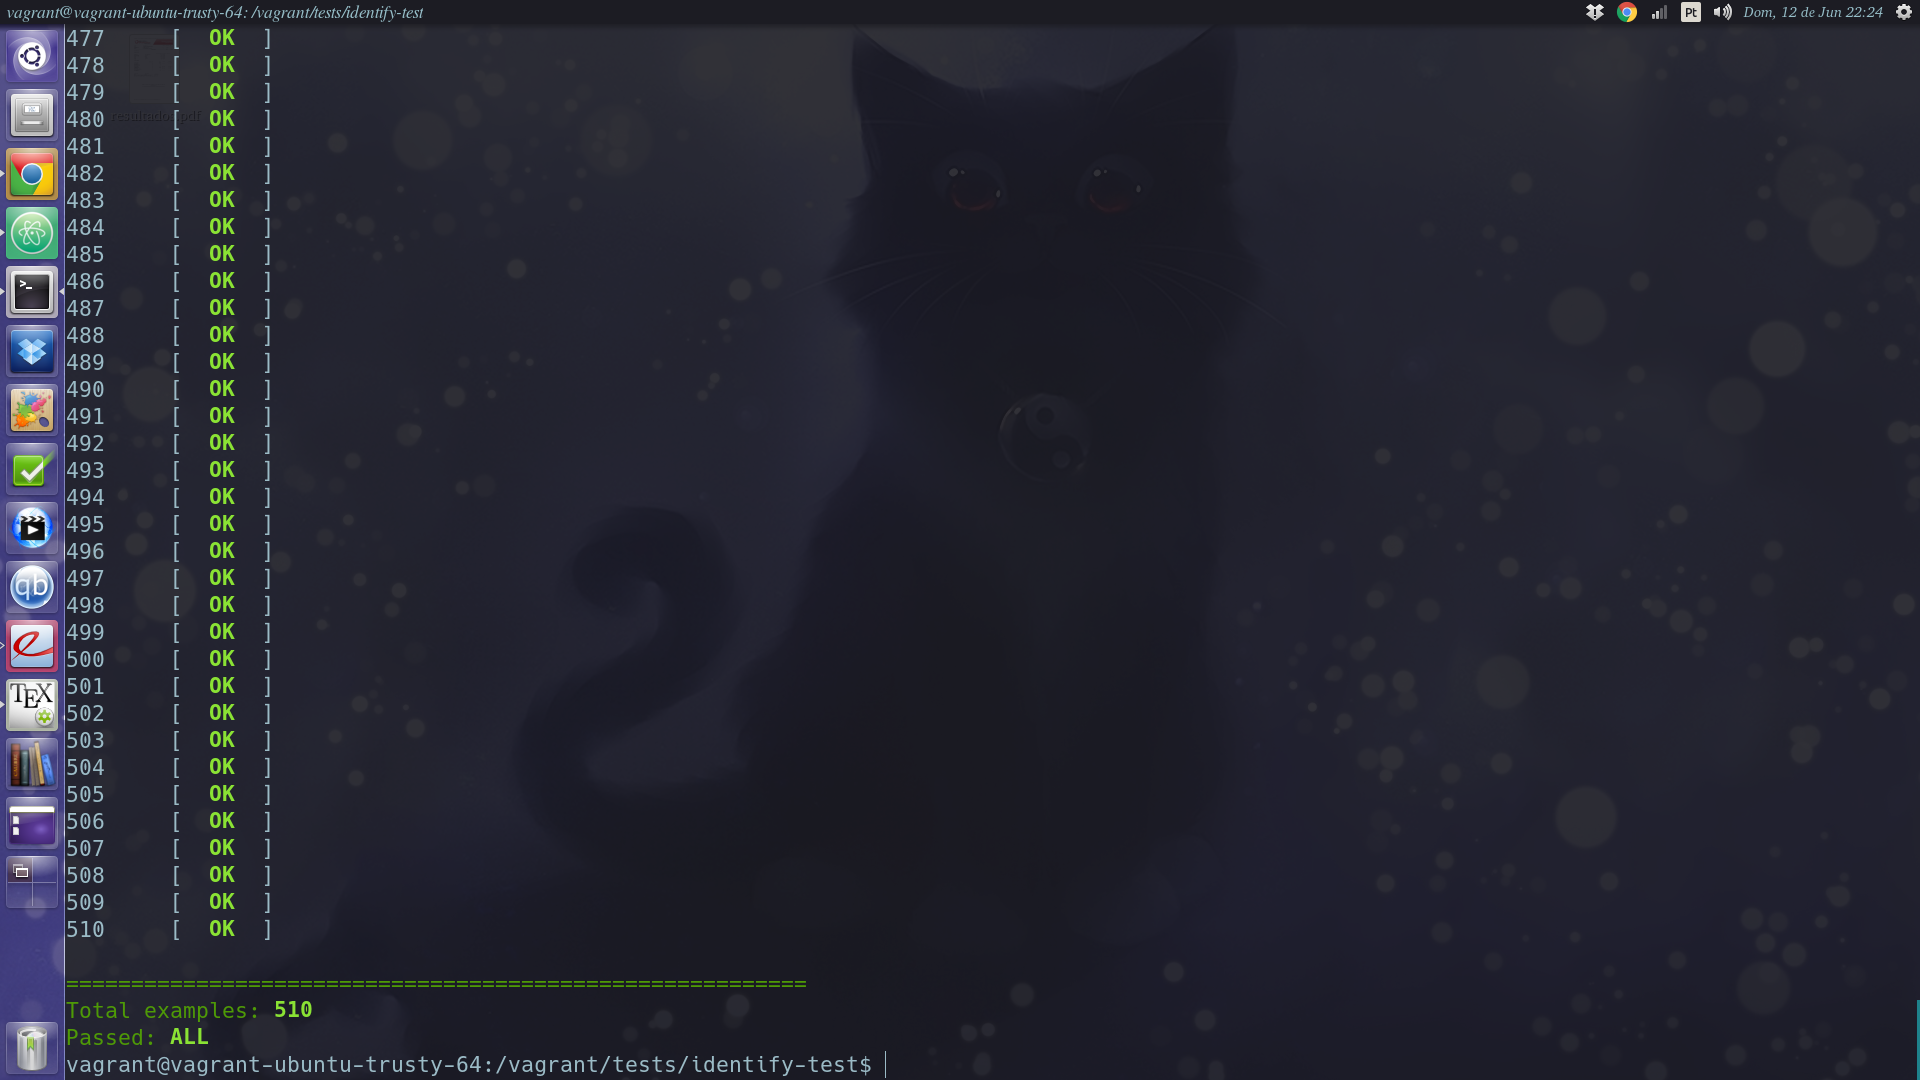
\includegraphics[width=0.8\textwidth]{figuras/identification-test.png}
    \caption{Resultado da execução do \textit{script} de teste de identificação}
    \label{identification-test}
\end{figure}
\FloatBarrier

Como evidenciado na Figura \ref{identification-test} o \parser passou numa
bateria de mais de 500 tentativas de identificação de regras em diversas
combinações.